


\tikzset{every picture/.style={line width=0.75pt}} %set default line width to 0.75pt        

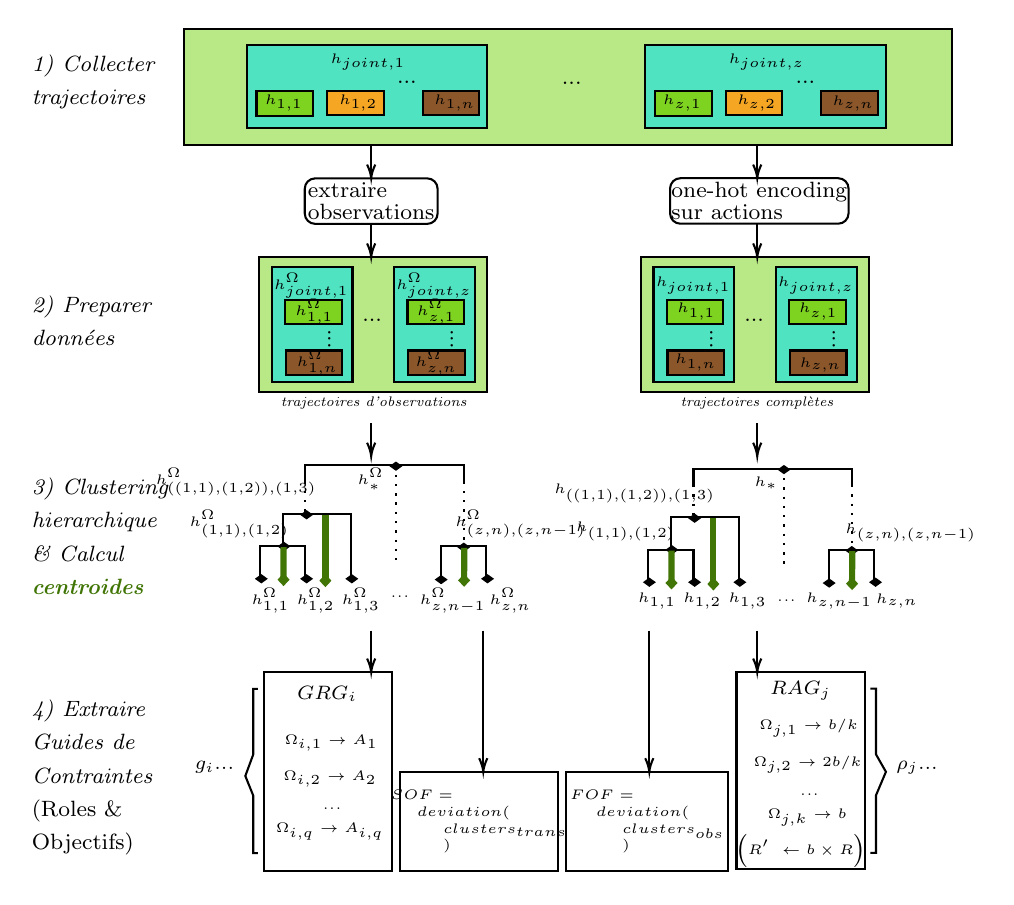
\begin{tikzpicture}[x=0.75pt,y=0.75pt,yscale=-1,xscale=1]
    %uncomment if require: \path (0,3196); %set diagram left start at 0, and has height of 3196

    %Shape: Rectangle [id:dp6446774683746603] 
    \draw  [fill={rgb, 255:red, 184; green, 233; blue, 134 }  ,fill opacity=1 ] (184,2054) -- (554,2054) -- (554,2110) -- (184,2110) -- cycle ;
    %Shape: Rectangle [id:dp11954381835057803] 
    \draw  [fill={rgb, 255:red, 80; green, 227; blue, 194 }  ,fill opacity=1 ] (214,2062) -- (330,2062) -- (330,2102) -- (214,2102) -- cycle ;
    %Shape: Rectangle [id:dp16354412692751719] 
    \draw  [fill={rgb, 255:red, 245; green, 166; blue, 35 }  ,fill opacity=1 ] (252.76,2083.89) -- (280,2083.89) -- (280,2095.6) -- (252.76,2095.6) -- cycle ;
    %Shape: Rectangle [id:dp2654297895337838] 
    \draw  [fill={rgb, 255:red, 139; green, 87; blue, 42 }  ,fill opacity=1 ] (298.76,2083.87) -- (326,2083.87) -- (326,2095.59) -- (298.76,2095.59) -- cycle ;
    %Shape: Rectangle [id:dp8985818084992432] 
    \draw  [fill={rgb, 255:red, 126; green, 211; blue, 33 }  ,fill opacity=1 ] (218.76,2084.16) -- (246,2084.16) -- (246,2095.87) -- (218.76,2095.87) -- cycle ;
    %Shape: Rectangle [id:dp48712472547976826] 
    \draw  [fill={rgb, 255:red, 255; green, 255; blue, 255 }  ,fill opacity=1 ] (242,2131.08) .. controls (242,2128.32) and (244.24,2126.08) .. (247,2126.08) -- (301,2126.08) .. controls (303.76,2126.08) and (306,2128.32) .. (306,2131.08) -- (306,2143) .. controls (306,2145.76) and (303.76,2148) .. (301,2148) -- (247,2148) .. controls (244.24,2148) and (242,2145.76) .. (242,2143) -- cycle ;

    %Shape: Rectangle [id:dp9481830819072239] 
    \draw  [fill={rgb, 255:red, 184; green, 233; blue, 134 }  ,fill opacity=1 ] (220,2164) -- (330,2164) -- (330,2229) -- (220,2229) -- cycle ;
    %Shape: Rectangle [id:dp41481109128799265] 
    \draw  [fill={rgb, 255:red, 80; green, 227; blue, 194 }  ,fill opacity=1 ] (226,2169) -- (265,2169) -- (265,2224) -- (226,2224) -- cycle ;
    %Shape: Rectangle [id:dp36210081179115716] 
    \draw  [fill={rgb, 255:red, 139; green, 87; blue, 42 }  ,fill opacity=1 ] (232.76,2209) -- (260,2209) -- (260,2220.71) -- (232.76,2220.71) -- cycle ;
    %Shape: Rectangle [id:dp9574972109935381] 
    \draw  [fill={rgb, 255:red, 126; green, 211; blue, 33 }  ,fill opacity=1 ] (232.48,2184.62) -- (259.72,2184.62) -- (259.72,2196.33) -- (232.48,2196.33) -- cycle ;
    %Shape: Rectangle [id:dp6763939878516604] 
    \draw  [fill={rgb, 255:red, 80; green, 227; blue, 194 }  ,fill opacity=1 ] (285,2169) -- (324,2169) -- (324,2224) -- (285,2224) -- cycle ;
    %Shape: Rectangle [id:dp7254457331732914] 
    \draw  [fill={rgb, 255:red, 139; green, 87; blue, 42 }  ,fill opacity=1 ] (291.76,2209) -- (319,2209) -- (319,2220.71) -- (291.76,2220.71) -- cycle ;
    %Shape: Rectangle [id:dp09098875701220999] 
    \draw  [fill={rgb, 255:red, 126; green, 211; blue, 33 }  ,fill opacity=1 ] (291.48,2184.62) -- (318.72,2184.62) -- (318.72,2196.33) -- (291.48,2196.33) -- cycle ;
    %Straight Lines [id:da310649499986848] 
    \draw    (220.53,2319) -- (220.53,2303.39) -- (242.33,2303.39) -- (242.33,2319) ;
    %Straight Lines [id:da4779343766066969] 
    \draw    (231.43,2303.39) -- (231.43,2287.77) -- (264.12,2287.77) -- (264.12,2319) ;
    %Straight Lines [id:da5756029666044655] 
    \draw    (242.33,2272.16) -- (242.33,2264.35) -- (318.61,2264.35) -- (318.61,2272.16) ;
    %Straight Lines [id:da000745643490450365] 
    \draw    (307.71,2319) -- (307.71,2303.39) -- (329.51,2303.39) -- (329.51,2319) ;
    %Shape: Ellipse [id:dp7156214883304655] 
    \draw  [line width=2.25]  (220.53,2319) .. controls (220.53,2318.79) and (220.78,2318.61) .. (221.08,2318.61) .. controls (221.38,2318.61) and (221.62,2318.79) .. (221.62,2319) .. controls (221.62,2319.22) and (221.38,2319.39) .. (221.08,2319.39) .. controls (220.78,2319.39) and (220.53,2319.22) .. (220.53,2319) -- cycle ;
    %Shape: Ellipse [id:dp3858567279639801] 
    \draw  [line width=2.25]  (242.33,2319) .. controls (242.33,2318.79) and (242.57,2318.61) .. (242.87,2318.61) .. controls (243.17,2318.61) and (243.42,2318.79) .. (243.42,2319) .. controls (243.42,2319.22) and (243.17,2319.39) .. (242.87,2319.39) .. controls (242.57,2319.39) and (242.33,2319.22) .. (242.33,2319) -- cycle ;
    %Shape: Ellipse [id:dp06345412404985873] 
    \draw  [line width=2.25]  (264.12,2319) .. controls (264.12,2318.79) and (264.37,2318.61) .. (264.67,2318.61) .. controls (264.97,2318.61) and (265.21,2318.79) .. (265.21,2319) .. controls (265.21,2319.22) and (264.97,2319.39) .. (264.67,2319.39) .. controls (264.37,2319.39) and (264.12,2319.22) .. (264.12,2319) -- cycle ;
    %Shape: Ellipse [id:dp23438755375160103] 
    \draw  [line width=2.25]  (307.17,2319.39) .. controls (307.17,2319.18) and (307.41,2319) .. (307.71,2319) .. controls (308.01,2319) and (308.26,2319.18) .. (308.26,2319.39) .. controls (308.26,2319.61) and (308.01,2319.78) .. (307.71,2319.78) .. controls (307.41,2319.78) and (307.17,2319.61) .. (307.17,2319.39) -- cycle ;
    %Shape: Ellipse [id:dp9125729527443308] 
    \draw  [line width=2.25]  (329.51,2319) .. controls (329.51,2318.79) and (329.75,2318.61) .. (330.05,2318.61) .. controls (330.35,2318.61) and (330.6,2318.79) .. (330.6,2319) .. controls (330.6,2319.22) and (330.35,2319.39) .. (330.05,2319.39) .. controls (329.75,2319.39) and (329.51,2319.22) .. (329.51,2319) -- cycle ;
    %Shape: Ellipse [id:dp9368497404716122] 
    \draw  [line width=2.25]  (231.43,2303.39) .. controls (231.43,2303.17) and (231.67,2303) .. (231.97,2303) .. controls (232.27,2303) and (232.52,2303.17) .. (232.52,2303.39) .. controls (232.52,2303.6) and (232.27,2303.78) .. (231.97,2303.78) .. controls (231.67,2303.78) and (231.43,2303.6) .. (231.43,2303.39) -- cycle ;
    %Shape: Ellipse [id:dp9082840601009624] 
    \draw  [line width=2.25]  (242.33,2288.16) .. controls (242.33,2287.95) and (242.57,2287.77) .. (242.87,2287.77) .. controls (243.17,2287.77) and (243.42,2287.95) .. (243.42,2288.16) .. controls (243.42,2288.38) and (243.17,2288.55) .. (242.87,2288.55) .. controls (242.57,2288.55) and (242.33,2288.38) .. (242.33,2288.16) -- cycle ;
    %Shape: Ellipse [id:dp9572066005117809] 
    \draw  [line width=2.25]  (285.37,2264.74) .. controls (285.37,2264.52) and (285.62,2264.35) .. (285.92,2264.35) .. controls (286.22,2264.35) and (286.46,2264.52) .. (286.46,2264.74) .. controls (286.46,2264.95) and (286.22,2265.13) .. (285.92,2265.13) .. controls (285.62,2265.13) and (285.37,2264.95) .. (285.37,2264.74) -- cycle ;
    %Shape: Ellipse [id:dp739566639462307] 
    \draw  [line width=2.25]  (318.06,2303.78) .. controls (318.06,2303.56) and (318.31,2303.39) .. (318.61,2303.39) .. controls (318.91,2303.39) and (319.15,2303.56) .. (319.15,2303.78) .. controls (319.15,2303.99) and (318.91,2304.17) .. (318.61,2304.17) .. controls (318.31,2304.17) and (318.06,2303.99) .. (318.06,2303.78) -- cycle ;
    %Straight Lines [id:da36201621077359325] 
    \draw  [dash pattern={on 0.84pt off 2.51pt}]  (242.33,2272.16) -- (242.33,2287.77) ;
    %Straight Lines [id:da3740526131455012] 
    \draw  [dash pattern={on 0.84pt off 2.51pt}]  (318.61,2272.16) -- (318.61,2303.39) ;
    %Straight Lines [id:da33114151268319136] 
    \draw  [dash pattern={on 0.84pt off 2.51pt}]  (285.92,2264.35) -- (285.92,2311.19) ;
    %Straight Lines [id:da9611554132027019] 
    \draw    (407.49,2320.66) -- (407.49,2305.04) -- (429.28,2305.04) -- (429.28,2320.66) ;
    %Straight Lines [id:da5452608062724974] 
    \draw    (418.38,2305.04) -- (418.38,2289.42) -- (451.08,2289.42) -- (451.08,2320.66) ;
    %Straight Lines [id:da5268642881289671] 
    \draw    (429.28,2273.81) -- (429.28,2266) -- (505.56,2266) -- (505.56,2273.81) ;
    %Straight Lines [id:da05744469340801017] 
    \draw    (494.67,2320.66) -- (494.67,2305.04) -- (516.46,2305.04) -- (516.46,2320.66) ;
    %Shape: Ellipse [id:dp616447935630148] 
    \draw  [line width=2.25]  (407.49,2320.66) .. controls (407.49,2320.44) and (407.73,2320.27) .. (408.03,2320.27) .. controls (408.33,2320.27) and (408.58,2320.44) .. (408.58,2320.66) .. controls (408.58,2320.87) and (408.33,2321.05) .. (408.03,2321.05) .. controls (407.73,2321.05) and (407.49,2320.87) .. (407.49,2320.66) -- cycle ;
    %Shape: Ellipse [id:dp3777096214669222] 
    \draw  [line width=2.25]  (429.28,2320.66) .. controls (429.28,2320.44) and (429.52,2320.27) .. (429.83,2320.27) .. controls (430.13,2320.27) and (430.37,2320.44) .. (430.37,2320.66) .. controls (430.37,2320.87) and (430.13,2321.05) .. (429.83,2321.05) .. controls (429.52,2321.05) and (429.28,2320.87) .. (429.28,2320.66) -- cycle ;
    %Shape: Ellipse [id:dp8138542385543501] 
    \draw  [line width=2.25]  (451.08,2320.66) .. controls (451.08,2320.44) and (451.32,2320.27) .. (451.62,2320.27) .. controls (451.92,2320.27) and (452.17,2320.44) .. (452.17,2320.66) .. controls (452.17,2320.87) and (451.92,2321.05) .. (451.62,2321.05) .. controls (451.32,2321.05) and (451.08,2320.87) .. (451.08,2320.66) -- cycle ;
    %Shape: Ellipse [id:dp322481737659716] 
    \draw  [line width=2.25]  (494.12,2321.05) .. controls (494.12,2320.83) and (494.36,2320.66) .. (494.67,2320.66) .. controls (494.97,2320.66) and (495.21,2320.83) .. (495.21,2321.05) .. controls (495.21,2321.26) and (494.97,2321.44) .. (494.67,2321.44) .. controls (494.36,2321.44) and (494.12,2321.26) .. (494.12,2321.05) -- cycle ;
    %Shape: Ellipse [id:dp7676517098779699] 
    \draw  [line width=2.25]  (516.46,2320.66) .. controls (516.46,2320.44) and (516.7,2320.27) .. (517.01,2320.27) .. controls (517.31,2320.27) and (517.55,2320.44) .. (517.55,2320.66) .. controls (517.55,2320.87) and (517.31,2321.05) .. (517.01,2321.05) .. controls (516.7,2321.05) and (516.46,2320.87) .. (516.46,2320.66) -- cycle ;
    %Shape: Ellipse [id:dp1585224562411227] 
    \draw  [line width=2.25]  (418.38,2305.04) .. controls (418.38,2304.82) and (418.63,2304.65) .. (418.93,2304.65) .. controls (419.23,2304.65) and (419.47,2304.82) .. (419.47,2305.04) .. controls (419.47,2305.26) and (419.23,2305.43) .. (418.93,2305.43) .. controls (418.63,2305.43) and (418.38,2305.26) .. (418.38,2305.04) -- cycle ;
    %Shape: Ellipse [id:dp02834033002913927] 
    \draw  [line width=2.25]  (429.28,2289.81) .. controls (429.28,2289.6) and (429.52,2289.42) .. (429.83,2289.42) .. controls (430.13,2289.42) and (430.37,2289.6) .. (430.37,2289.81) .. controls (430.37,2290.03) and (430.13,2290.2) .. (429.83,2290.2) .. controls (429.52,2290.2) and (429.28,2290.03) .. (429.28,2289.81) -- cycle ;
    %Shape: Ellipse [id:dp9471335251053217] 
    \draw  [line width=2.25]  (472.33,2266.39) .. controls (472.33,2266.17) and (472.57,2266) .. (472.87,2266) .. controls (473.17,2266) and (473.42,2266.17) .. (473.42,2266.39) .. controls (473.42,2266.61) and (473.17,2266.78) .. (472.87,2266.78) .. controls (472.57,2266.78) and (472.33,2266.61) .. (472.33,2266.39) -- cycle ;
    %Shape: Ellipse [id:dp8036746049983543] 
    \draw  [line width=2.25]  (505.02,2305.43) .. controls (505.02,2305.21) and (505.26,2305.04) .. (505.56,2305.04) .. controls (505.86,2305.04) and (506.11,2305.21) .. (506.11,2305.43) .. controls (506.11,2305.65) and (505.86,2305.82) .. (505.56,2305.82) .. controls (505.26,2305.82) and (505.02,2305.65) .. (505.02,2305.43) -- cycle ;
    %Straight Lines [id:da4862783270480875] 
    \draw  [dash pattern={on 0.84pt off 2.51pt}]  (429.28,2273.81) -- (429.28,2289.42) ;
    %Straight Lines [id:da33705102258229946] 
    \draw  [dash pattern={on 0.84pt off 2.51pt}]  (505.56,2273.81) -- (505.56,2305.04) ;
    %Straight Lines [id:da7632784737841659] 
    \draw  [dash pattern={on 0.84pt off 2.51pt}]  (472.87,2266) -- (472.87,2312.85) ;
    %Shape: Rectangle [id:dp8486981747751949] 
    \draw  [fill={rgb, 255:red, 184; green, 233; blue, 134 }  ,fill opacity=1 ] (404,2164) -- (514,2164) -- (514,2229) -- (404,2229) -- cycle ;
    %Shape: Rectangle [id:dp8662345148113237] 
    \draw  [fill={rgb, 255:red, 80; green, 227; blue, 194 }  ,fill opacity=1 ] (410,2169) -- (449,2169) -- (449,2224) -- (410,2224) -- cycle ;
    %Shape: Rectangle [id:dp7401789100724447] 
    \draw  [fill={rgb, 255:red, 139; green, 87; blue, 42 }  ,fill opacity=1 ] (416.76,2209) -- (444,2209) -- (444,2220.71) -- (416.76,2220.71) -- cycle ;
    %Shape: Rectangle [id:dp732580883063841] 
    \draw  [fill={rgb, 255:red, 126; green, 211; blue, 33 }  ,fill opacity=1 ] (416.48,2184.62) -- (443.72,2184.62) -- (443.72,2196.33) -- (416.48,2196.33) -- cycle ;
    %Shape: Rectangle [id:dp9235809941782823] 
    \draw  [fill={rgb, 255:red, 80; green, 227; blue, 194 }  ,fill opacity=1 ] (469,2169) -- (508,2169) -- (508,2224) -- (469,2224) -- cycle ;
    %Shape: Rectangle [id:dp6899402027382165] 
    \draw  [fill={rgb, 255:red, 139; green, 87; blue, 42 }  ,fill opacity=1 ] (475.76,2209) -- (503,2209) -- (503,2220.71) -- (475.76,2220.71) -- cycle ;
    %Shape: Rectangle [id:dp17139392675097032] 
    \draw  [fill={rgb, 255:red, 126; green, 211; blue, 33 }  ,fill opacity=1 ] (475.48,2184.62) -- (502.72,2184.62) -- (502.72,2196.33) -- (475.48,2196.33) -- cycle ;
    %Straight Lines [id:da5226422691270944] 
    \draw [color={rgb, 255:red, 65; green, 117; blue, 5 }  ,draw opacity=1 ][line width=2.25]    (231.77,2320.33) -- (231.81,2303.78) ;
    %Shape: Ellipse [id:dp5047419290586512] 
    \draw  [color={rgb, 255:red, 65; green, 117; blue, 5 }  ,draw opacity=1 ][line width=2.25]  (230.92,2319.42) .. controls (230.92,2318.91) and (231.3,2318.5) .. (231.77,2318.5) .. controls (232.24,2318.5) and (232.63,2318.91) .. (232.63,2319.42) .. controls (232.63,2319.92) and (232.24,2320.33) .. (231.77,2320.33) .. controls (231.3,2320.33) and (230.92,2319.92) .. (230.92,2319.42) -- cycle ;
    %Straight Lines [id:da40145914360461865] 
    \draw [color={rgb, 255:red, 65; green, 117; blue, 5 }  ,draw opacity=1 ][line width=2.25]    (251.94,2319) -- (251.94,2288.17) ;
    %Shape: Ellipse [id:dp8858416104743969] 
    \draw  [color={rgb, 255:red, 65; green, 117; blue, 5 }  ,draw opacity=1 ][line width=2.25]  (251.08,2319.92) .. controls (251.08,2319.41) and (251.47,2319) .. (251.94,2319) .. controls (252.41,2319) and (252.79,2319.41) .. (252.79,2319.92) .. controls (252.79,2320.42) and (252.41,2320.83) .. (251.94,2320.83) .. controls (251.47,2320.83) and (251.08,2320.42) .. (251.08,2319.92) -- cycle ;
    %Straight Lines [id:da6353184164708716] 
    \draw [color={rgb, 255:red, 65; green, 117; blue, 5 }  ,draw opacity=1 ][line width=2.25]    (318.77,2320.67) -- (318.81,2304.11) ;
    %Shape: Ellipse [id:dp9629746335106062] 
    \draw  [color={rgb, 255:red, 65; green, 117; blue, 5 }  ,draw opacity=1 ][line width=2.25]  (317.92,2319.75) .. controls (317.92,2319.24) and (318.3,2318.83) .. (318.77,2318.83) .. controls (319.24,2318.83) and (319.63,2319.24) .. (319.63,2319.75) .. controls (319.63,2320.26) and (319.24,2320.67) .. (318.77,2320.67) .. controls (318.3,2320.67) and (317.92,2320.26) .. (317.92,2319.75) -- cycle ;
    %Straight Lines [id:da7403569117479297] 
    \draw [color={rgb, 255:red, 65; green, 117; blue, 5 }  ,draw opacity=1 ][line width=2.25]    (418.7,2321.94) -- (418.74,2305.38) ;
    %Shape: Ellipse [id:dp9693987957556999] 
    \draw  [color={rgb, 255:red, 65; green, 117; blue, 5 }  ,draw opacity=1 ][line width=2.25]  (417.84,2321.02) .. controls (417.84,2320.52) and (418.23,2320.11) .. (418.7,2320.11) .. controls (419.17,2320.11) and (419.56,2320.52) .. (419.56,2321.02) .. controls (419.56,2321.53) and (419.17,2321.94) .. (418.7,2321.94) .. controls (418.23,2321.94) and (417.84,2321.53) .. (417.84,2321.02) -- cycle ;
    %Straight Lines [id:da0840318719732559] 
    \draw [color={rgb, 255:red, 65; green, 117; blue, 5 }  ,draw opacity=1 ][line width=2.25]    (438.87,2320.61) -- (438.87,2289.77) ;
    %Shape: Ellipse [id:dp38103443949256577] 
    \draw  [color={rgb, 255:red, 65; green, 117; blue, 5 }  ,draw opacity=1 ][line width=2.25]  (438.01,2321.52) .. controls (438.01,2321.02) and (438.39,2320.61) .. (438.87,2320.61) .. controls (439.34,2320.61) and (439.72,2321.02) .. (439.72,2321.52) .. controls (439.72,2322.03) and (439.34,2322.44) .. (438.87,2322.44) .. controls (438.39,2322.44) and (438.01,2322.03) .. (438.01,2321.52) -- cycle ;
    %Straight Lines [id:da5025807566153033] 
    \draw [color={rgb, 255:red, 65; green, 117; blue, 5 }  ,draw opacity=1 ][line width=2.25]    (505.7,2322.27) -- (505.74,2305.72) ;
    %Shape: Ellipse [id:dp2054322761052696] 
    \draw  [color={rgb, 255:red, 65; green, 117; blue, 5 }  ,draw opacity=1 ][line width=2.25]  (504.84,2321.36) .. controls (504.84,2320.85) and (505.23,2320.44) .. (505.7,2320.44) .. controls (506.17,2320.44) and (506.56,2320.85) .. (506.56,2321.36) .. controls (506.56,2321.86) and (506.17,2322.27) .. (505.7,2322.27) .. controls (505.23,2322.27) and (504.84,2321.86) .. (504.84,2321.36) -- cycle ;
    %Shape: Rectangle [id:dp18036074660325163] 
    \draw   (222.17,2364) -- (284,2364) -- (284,2460) -- (222.17,2460) -- cycle ;
    %Shape: Rectangle [id:dp3757874344168871] 
    \draw   (450,2364) -- (511.83,2364) -- (511.83,2458.97) -- (450,2458.97) -- cycle ;
    %Straight Lines [id:da4807858714110206] 
    \draw    (514.51,2371.91) -- (517.2,2371.91) -- (517.2,2403.57) -- (522,2412) -- (517.2,2423.36) -- (517.2,2451.06) -- (514.51,2451.06) ;
    %Shape: Rectangle [id:dp6563270106594438] 
    \draw   (288,2412) -- (364,2412) -- (364,2460) -- (288,2460) -- cycle ;

    %Shape: Rectangle [id:dp3825654404747878] 
    \draw  [fill={rgb, 255:red, 80; green, 227; blue, 194 }  ,fill opacity=1 ] (406,2062) -- (522,2062) -- (522,2102) -- (406,2102) -- cycle ;
    %Shape: Rectangle [id:dp973718882488827] 
    \draw  [fill={rgb, 255:red, 245; green, 166; blue, 35 }  ,fill opacity=1 ] (444.76,2083.89) -- (472,2083.89) -- (472,2095.6) -- (444.76,2095.6) -- cycle ;
    %Shape: Rectangle [id:dp0248437668015975] 
    \draw  [fill={rgb, 255:red, 139; green, 87; blue, 42 }  ,fill opacity=1 ] (490.76,2083.87) -- (518,2083.87) -- (518,2095.59) -- (490.76,2095.59) -- cycle ;
    %Shape: Rectangle [id:dp3173994637780163] 
    \draw  [fill={rgb, 255:red, 126; green, 211; blue, 33 }  ,fill opacity=1 ] (410.76,2084.16) -- (438,2084.16) -- (438,2095.87) -- (410.76,2095.87) -- cycle ;
    %Straight Lines [id:da44145788537292463] 
    \draw    (274,2110) -- (274,2124) ;
    \draw [shift={(274,2126)}, rotate = 270] [color={rgb, 255:red, 0; green, 0; blue, 0 }  ][line width=0.75]    (6.56,-1.97) .. controls (4.17,-0.84) and (1.99,-0.18) .. (0,0) .. controls (1.99,0.18) and (4.17,0.84) .. (6.56,1.97)   ;
    %Straight Lines [id:da006646172117977911] 
    \draw    (274,2148) -- (274,2162) ;
    \draw [shift={(274,2164)}, rotate = 270] [color={rgb, 255:red, 0; green, 0; blue, 0 }  ][line width=0.75]    (6.56,-1.97) .. controls (4.17,-0.84) and (1.99,-0.18) .. (0,0) .. controls (1.99,0.18) and (4.17,0.84) .. (6.56,1.97)   ;
    %Shape: Rectangle [id:dp5947531945722148] 
    \draw  [fill={rgb, 255:red, 255; green, 255; blue, 255 }  ,fill opacity=1 ] (418,2131) .. controls (418,2128.24) and (420.24,2126) .. (423,2126) -- (499,2126) .. controls (501.76,2126) and (504,2128.24) .. (504,2131) -- (504,2142.92) .. controls (504,2145.68) and (501.76,2147.92) .. (499,2147.92) -- (423,2147.92) .. controls (420.24,2147.92) and (418,2145.68) .. (418,2142.92) -- cycle ;

    %Straight Lines [id:da1469916019080323] 
    \draw    (460,2110) -- (460,2124) ;
    \draw [shift={(460,2126)}, rotate = 270] [color={rgb, 255:red, 0; green, 0; blue, 0 }  ][line width=0.75]    (6.56,-1.97) .. controls (4.17,-0.84) and (1.99,-0.18) .. (0,0) .. controls (1.99,0.18) and (4.17,0.84) .. (6.56,1.97)   ;
    %Straight Lines [id:da48571688709823413] 
    \draw    (460,2148) -- (460,2162) ;
    \draw [shift={(460,2164)}, rotate = 270] [color={rgb, 255:red, 0; green, 0; blue, 0 }  ][line width=0.75]    (6.56,-1.97) .. controls (4.17,-0.84) and (1.99,-0.18) .. (0,0) .. controls (1.99,0.18) and (4.17,0.84) .. (6.56,1.97)   ;
    %Straight Lines [id:da10082879672889511] 
    \draw    (274,2244) -- (274,2258) ;
    \draw [shift={(274,2260)}, rotate = 270] [color={rgb, 255:red, 0; green, 0; blue, 0 }  ][line width=0.75]    (6.56,-1.97) .. controls (4.17,-0.84) and (1.99,-0.18) .. (0,0) .. controls (1.99,0.18) and (4.17,0.84) .. (6.56,1.97)   ;
    %Straight Lines [id:da6259013142611769] 
    \draw    (460,2244) -- (460,2258) ;
    \draw [shift={(460,2260)}, rotate = 270] [color={rgb, 255:red, 0; green, 0; blue, 0 }  ][line width=0.75]    (6.56,-1.97) .. controls (4.17,-0.84) and (1.99,-0.18) .. (0,0) .. controls (1.99,0.18) and (4.17,0.84) .. (6.56,1.97)   ;
    %Straight Lines [id:da37112437512887253] 
    \draw    (274,2344) -- (274,2362) ;
    \draw [shift={(274,2364)}, rotate = 270] [color={rgb, 255:red, 0; green, 0; blue, 0 }  ][line width=0.75]    (6.56,-1.97) .. controls (4.17,-0.84) and (1.99,-0.18) .. (0,0) .. controls (1.99,0.18) and (4.17,0.84) .. (6.56,1.97)   ;
    %Straight Lines [id:da7692948858201427] 
    \draw    (460,2344) -- (460,2362) ;
    \draw [shift={(460,2364)}, rotate = 270] [color={rgb, 255:red, 0; green, 0; blue, 0 }  ][line width=0.75]    (6.56,-1.97) .. controls (4.17,-0.84) and (1.99,-0.18) .. (0,0) .. controls (1.99,0.18) and (4.17,0.84) .. (6.56,1.97)   ;
    %Straight Lines [id:da08711296960205606] 
    \draw    (219.42,2372) -- (217.17,2372) -- (217.17,2403.66) -- (213.36,2414) -- (217.17,2423.44) -- (217.17,2451.14) -- (219.42,2451.14) ;
    %Straight Lines [id:da7520506466890287] 
    \draw    (328,2344) -- (328,2410) ;
    \draw [shift={(328,2412)}, rotate = 270] [color={rgb, 255:red, 0; green, 0; blue, 0 }  ][line width=0.75]    (6.56,-1.97) .. controls (4.17,-0.84) and (1.99,-0.18) .. (0,0) .. controls (1.99,0.18) and (4.17,0.84) .. (6.56,1.97)   ;
    %Straight Lines [id:da2882853294833533] 
    \draw    (408,2344) -- (408,2410) ;
    \draw [shift={(408,2412)}, rotate = 270] [color={rgb, 255:red, 0; green, 0; blue, 0 }  ][line width=0.75]    (6.56,-1.97) .. controls (4.17,-0.84) and (1.99,-0.18) .. (0,0) .. controls (1.99,0.18) and (4.17,0.84) .. (6.56,1.97)   ;
    %Shape: Rectangle [id:dp6985462910267374] 
    \draw   (368,2412) -- (446,2412) -- (446,2460) -- (368,2460) -- cycle ;



    % Text Node
    \draw (198.5,2410) node  [font=\scriptsize] [align=left] {$\displaystyle g_{i} ...$};
    % Text Node
    \draw (506.31,2090) node  [font=\tiny] [align=left] {$\displaystyle h_{z,n}$};
    % Text Node
    \draw (459.81,2089.87) node  [font=\tiny] [align=left] {$\displaystyle h_{z,2}$};
    % Text Node
    \draw (424,2090) node  [font=\tiny] [align=left] {$\displaystyle h_{z,1}$};
    % Text Node
    \draw (464.5,2070) node  [font=\tiny] [align=left] {$\displaystyle h_{joint,z}$};
    % Text Node
    \draw (473.76,2077.87) node [anchor=north west][inner sep=0.75pt]  [font=\footnotesize] [align=left] {\begin{minipage}[lt]{9.53pt}\setlength\topsep{0pt}
            \begin{flushright}
                ...
            \end{flushright}

        \end{minipage}};
    % Text Node
    \draw (480.89,2450.23) node  [font=\tiny] [align=left] {$\displaystyle \left( R'\ \leftarrow b\times R\right)$};
    % Text Node
    \draw (485.18,2422.87) node  [font=\tiny] [align=left] {$\displaystyle ...$};
    % Text Node
    \draw (484.08,2434.13) node  [font=\tiny] [align=left] {$\displaystyle \Omega _{j,k}\rightarrow b$};
    % Text Node
    \draw (484.28,2408.5) node  [font=\tiny] [align=left] {$\displaystyle \Omega _{j,2}\rightarrow 2b/k$};
    % Text Node
    \draw (484.81,2390.97) node  [font=\tiny] [align=left] {$\displaystyle \Omega _{j,1}\rightarrow b/k$};
    % Text Node
    \draw (255.17,2429.74) node  [font=\tiny] [align=left] {$\displaystyle ...$};
    % Text Node
    \draw (254.07,2440.88) node  [font=\tiny] [align=left] {$\displaystyle \Omega _{i,q}\rightarrow A_{i,q}$};
    % Text Node
    \draw (254.27,2415.52) node  [font=\tiny] [align=left] {$\displaystyle \Omega _{i,2}\rightarrow A_{2}$};
    % Text Node
    \draw (254.8,2398.16) node  [font=\tiny] [align=left] {$\displaystyle \Omega _{i,1}\rightarrow A_{1}$};
    % Text Node
    \draw (537,2410) node  [font=\scriptsize] [align=left] {$\displaystyle \rho _{j} ...$};
    % Text Node
    \draw (252.79,2374.51) node  [font=\scriptsize] [align=left] {$\displaystyle GRG_{i}$};
    % Text Node
    \draw (480.89,2372.97) node  [font=\scriptsize] [align=left] {$\displaystyle RAG_{j}$};
    % Text Node
    \draw (460.18,2234.5) node   [align=left] {{\tiny \textit{trajectoires complètes}}};
    % Text Node
    \draw (275.5,2234.5) node   [align=left] {{\tiny \textit{trajectoires d'observations}}};
    % Text Node
    \draw (448.99,2195.53) node [anchor=west] [inner sep=0.75pt]  [font=\footnotesize] [align=left] {\begin{minipage}[lt]{9.53pt}\setlength\topsep{0pt}
            \begin{flushright}
                ...
            \end{flushright}

        \end{minipage}};
    % Text Node
    \draw (490.5,2216.03) node  [font=\tiny] [align=left] {$\displaystyle h_{z,n}$};
    % Text Node
    \draw (489.45,2190.24) node  [font=\tiny] [align=left] {$\displaystyle h_{z,1}$};
    % Text Node
    \draw (488.23,2177.83) node  [font=\tiny] [align=left] {$\displaystyle h_{joint,z}$};
    % Text Node
    \draw (499,2194) node [anchor=north west][inner sep=0.75pt]  [font=\footnotesize,rotate=-90] [align=left] {\begin{minipage}[lt]{9.53pt}\setlength\topsep{0pt}
            \begin{flushright}
                ...
            \end{flushright}

        \end{minipage}};
    % Text Node
    \draw (430.38,2214.86) node  [font=\tiny] [align=left] {$\displaystyle h_{1,n}$};
    % Text Node
    \draw (430.69,2190.24) node  [font=\tiny] [align=left] {$\displaystyle h_{1,1}$};
    % Text Node
    \draw (429.22,2177.83) node  [font=\tiny] [align=left] {$\displaystyle h_{joint,1}$};
    % Text Node
    \draw (440,2194) node [anchor=north west][inner sep=0.75pt]  [font=\footnotesize,rotate=-90] [align=left] {\begin{minipage}[lt]{9.53pt}\setlength\topsep{0pt}
            \begin{flushright}
                ...
            \end{flushright}

        \end{minipage}};
    % Text Node
    \draw (109,2376) node [anchor=north west][inner sep=0.75pt]   [align=left] {{\footnotesize \textit{4) Extraire}}\\{\footnotesize \textit{Guides de}}\\{\footnotesize \textit{Contraintes}}\\{\footnotesize (Roles \&}\\{\footnotesize Objectifs)}};
    % Text Node
    \draw (109,2269) node [anchor=north west][inner sep=0.75pt]   [align=left] {{\footnotesize \textit{3) Clustering}}\\{\footnotesize \textit{hierarchique}}\\{\footnotesize \textit{\& Calcul}}\\{\footnotesize \textit{\textcolor[rgb]{0.25,0.46,0.02}{\textbf{centroides}}}}};
    % Text Node
    \draw (109,2181) node [anchor=north west][inner sep=0.75pt]   [align=left] {{\footnotesize \textit{2) Preparer}}\\{\footnotesize \textit{données}}};
    % Text Node
    \draw (109,2065) node [anchor=north west][inner sep=0.75pt]   [align=left] {{\footnotesize \textit{1) Collecter}}\\{\footnotesize \textit{trajectoires}}};
    % Text Node
    \draw (346,2292.59) node  [font=\tiny] [align=left] {$\displaystyle h_{( z,n) ,( z,n-1)}^{\Omega }$};
    % Text Node
    \draw (266,2264.27) node [anchor=north west][inner sep=0.75pt]  [font=\tiny] [align=left] {$\displaystyle h_{*}^{\Omega }$};
    % Text Node
    \draw (209,2272.59) node  [font=\tiny] [align=left] {$\displaystyle h_{(( 1,1) ,( 1,2)) ,( 1,3)}^{\Omega }$};
    % Text Node
    \draw (210.5,2292.59) node  [font=\tiny] [align=left] {$\displaystyle h_{( 1,1) ,( 1,2)}^{\Omega }$};
    % Text Node
    \draw (341.01,2329.5) node  [font=\tiny] [align=left] {$\displaystyle h_{z,n}^{\Omega }$};
    % Text Node
    \draw (313.32,2329.5) node  [font=\tiny] [align=left] {$\displaystyle h_{z,n-1}^{\Omega }$};
    % Text Node
    \draw (287.82,2327.74) node  [font=\tiny] [align=left] {$\displaystyle ...$};
    % Text Node
    \draw (269.09,2329.5) node  [font=\tiny] [align=left] {$\displaystyle h_{1,3}^{\Omega }$};
    % Text Node
    \draw (247.3,2329.5) node  [font=\tiny] [align=left] {$\displaystyle h_{1,2}^{\Omega }$};
    % Text Node
    \draw (225.5,2329.5) node  [font=\tiny] [align=left] {$\displaystyle h_{1,1}^{\Omega }$};
    % Text Node
    \draw (534,2296.84) node  [font=\tiny] [align=left] {$\displaystyle h_{( z,n) ,( z,n-1)}$};
    % Text Node
    \draw (464.26,2272.93) node  [font=\tiny] [align=left] {$\displaystyle h_{*}$};
    % Text Node
    \draw (401,2278) node  [font=\tiny] [align=left] {$\displaystyle h_{(( 1,1) ,( 1,2)) ,( 1,3)}$};
    % Text Node
    \draw (396.71,2296.07) node  [font=\tiny] [align=left] {$\displaystyle h_{( 1,1) ,( 1,2)}$};
    % Text Node
    \draw (527.28,2329.77) node  [font=\tiny] [align=left] {$\displaystyle h_{z,n}$};
    % Text Node
    \draw (499.58,2329.77) node  [font=\tiny] [align=left] {$\displaystyle h_{z,n-1}$};
    % Text Node
    \draw (474.09,2329.39) node  [font=\tiny] [align=left] {$\displaystyle ...$};
    % Text Node
    \draw (455.35,2329.77) node  [font=\tiny] [align=left] {$\displaystyle h_{1,3}$};
    % Text Node
    \draw (433.56,2329.77) node  [font=\tiny] [align=left] {$\displaystyle h_{1,2}$};
    % Text Node
    \draw (411.76,2329.77) node  [font=\tiny] [align=left] {$\displaystyle h_{1,1}$};
    % Text Node
    \draw (264.99,2195.53) node [anchor=west] [inner sep=0.75pt]  [font=\footnotesize] [align=left] {\begin{minipage}[lt]{9.53pt}\setlength\topsep{0pt}
            \begin{flushright}
                ...
            \end{flushright}

        \end{minipage}};
    % Text Node
    \draw (305.38,2214.86) node  [font=\tiny] [align=left] {$\displaystyle h_{z,n}^{\Omega }$};
    % Text Node
    \draw (305.45,2190.24) node  [font=\tiny] [align=left] {$\displaystyle h_{z,1}^{\Omega }$};
    % Text Node
    \draw (304.23,2177.83) node  [font=\tiny] [align=left] {$\displaystyle h_{joint,z}^{\Omega }$};
    % Text Node
    \draw (315,2194) node [anchor=north west][inner sep=0.75pt]  [font=\footnotesize,rotate=-90] [align=left] {\begin{minipage}[lt]{9.53pt}\setlength\topsep{0pt}
            \begin{flushright}
                ...
            \end{flushright}

        \end{minipage}};
    % Text Node
    \draw (248,2215) node  [font=\tiny] [align=left] {$\displaystyle h_{1,n}^{\Omega }$};
    % Text Node
    \draw (246.69,2190.24) node  [font=\tiny] [align=left] {$\displaystyle h_{1,1}^{\Omega }$};
    % Text Node
    \draw (245.22,2177.83) node  [font=\tiny] [align=left] {$\displaystyle h_{joint,1}^{\Omega }$};
    % Text Node
    \draw (256,2194) node [anchor=north west][inner sep=0.75pt]  [font=\footnotesize,rotate=-90] [align=left] {\begin{minipage}[lt]{9.53pt}\setlength\topsep{0pt}
            \begin{flushright}
                ...
            \end{flushright}

        \end{minipage}};
    % Text Node
    \draw (314.31,2090) node  [font=\tiny] [align=left] {$\displaystyle h_{1,n}$};
    % Text Node
    \draw (267.81,2089.87) node  [font=\tiny] [align=left] {$\displaystyle h_{1,2}$};
    % Text Node
    \draw (232,2090) node  [font=\tiny] [align=left] {$\displaystyle h_{1,1}$};
    % Text Node
    \draw (272.5,2070) node  [font=\tiny] [align=left] {$\displaystyle h_{joint,1}$};
    % Text Node
    \draw (281.76,2077.87) node [anchor=north west][inner sep=0.75pt]  [font=\footnotesize] [align=left] {\begin{minipage}[lt]{9.53pt}\setlength\topsep{0pt}
            \begin{flushright}
                ...
            \end{flushright}

        \end{minipage}};
    % Text Node
    \draw (369,2081.5) node  [font=\footnotesize] [align=left] {\begin{minipage}[lt]{9.53pt}\setlength\topsep{0pt}
            \begin{flushright}
                ...
            \end{flushright}

        \end{minipage}};
    % Text Node
    \draw (407,2436) node  [font=\tiny] [align=left] {$\displaystyle  \begin{array}{{>{\displaystyle}l}}
                FOF=                           \\
                \ \ \ \ deviation(             \\
                \ \ \ \ \ \ \ \ clusters_{obs} \\
                \ \ \ \ \ \ \ \ \dotsc )
            \end{array}$};
    % Text Node
    \draw (461,2136.96) node  [font=\scriptsize] [align=left] {{\footnotesize one-hot encoding}\\{\footnotesize sur actions}};
    % Text Node
    \draw (326,2436) node  [font=\tiny] [align=left] {$\displaystyle  \begin{array}{{>{\displaystyle}l}}
                SOF=                             \\
                \ \ \ \ deviation(               \\
                \ \ \ \ \ \ \ \ clusters_{trans} \\
                \ \ \ \ \ \ \ \ \dotsc )
            \end{array}$};
    % Text Node
    \draw (274,2137.04) node  [font=\scriptsize] [align=left] {{\footnotesize extraire}\\{\footnotesize observations}};


\end{tikzpicture}